\documentclass[tikz, border=5pt]{thesis}

\usepackage[edges]{forest}

\title{Data Storage and Serving Architecture for HTRC Corpus}
\author{HTRC IU Team}

\begin{document}

\maketitle

\tableofcontents

\begin{abstract}
TBD.
\end{abstract}

\section{Introduction}
With the recent acquisition of full Hathitrust corpus of 13.8 million digitized volumes, HTRC is working towards providing non-consumptive access to the full corpus. HTRC stores the corpus in IU Data Capacitor 2 structured according to pairtree~\cite{pairtree} file system heirarchy. Also, there is a copy of pairtree content packed into binary blobs that work with a in-house data processing and serving solution for HPC.

Data Capsules enable non-consumptive access to HTRC corpus and HTRC serves data to Data Capsules via the Data API~\cite{dataapi} which is a REST service backed by a Cassandra cluster. Current Data API provides access to a part of the full corpus, which is about 4 million digitized volumes.

HTRC aims to provide non-consumptive access to full Hathitrust corpus in coming months and this document discusses requirements -- both functional and non functional, data models, and solutions for enabling non-consumptive access to full corpus efficiently.

In addition to serving the full corpus via Data API, we are envisioning the use of Big Data frameworks such as Hadoop and Spark to process the corpus. This document will also address future use cases similar to mention above as well.

\section{Requirements}

\begin{itemize}
	\item Serve the full corpus via a REST API (Data API)
	\item 
	page level access 
	\item Read throughput of the system should be sufficient to utilize at least 50\% or more of the 40Gb/s network link
	\item An API to check the availability of volumes
	\item Access to volume metadata via REST API
	\item Enable processing the corpus using Big Data frameworks such as Hadoop and Spark
\end{itemize}
    
\section{Data Models}

\subsection{Raw Data}

For each raw volume, we have a \texttt{<volume-id>.mets.xml} containing all the volume metadata including page information and a \texttt{<volume-id>.zip} file containing the OCRed content. The zip file contains all the individual pages defined in the mets file as well as a single text file which is a concatenation of all the pages.

\begin{forest}
  for tree={%
    folder,
    grow'=0,
    fit=band
  }
    [<vol-id>
      [<vol-id>.mets.xml]
      [<vol-id>.zip
        [<vol-id>
          [00000001.txt]
          [00000002.txt]
          [...]
          [00000266.txt]]]]
\end{forest}


\subsection{Data API}

Data API will respond with a ZIP file containing volume content in following format upon a request with a list of volumes ids (\texttt{inu.3011012|uc2.ark:/13960/t2qxv15}) or a list of pages ids (\texttt{inu.3011012[1,2,20,30]|uc2.ark:/13960/t2qxv15[11,45\\,30,17,22,55]}).

\begin{forest}
  for tree={%
    folder,
    grow'=0,
    fit=band
  }
[volumes.zip
  [inu.3011012
  	[00000001.txt]
  	[00000002.txt]
  	[00000020.txt]
  	[00000030.txt]
  	[mets.xml]]
  [uc2.ark:/13960/t2qxv15
    [00000011.txt]
    [00000045.txt]
    [00000030.txt]
    [00000017.txt]
    [00000022.txt]
    [00000055.txt]
    [mets.xml]]]
\end{forest}

In addition to above Data API sends back concatenated text content if user requests the output to be concatenated.

\subsection{Storage}

    
\section{Discussion Notes}

\begin{figure}[ht!]
    \centering
    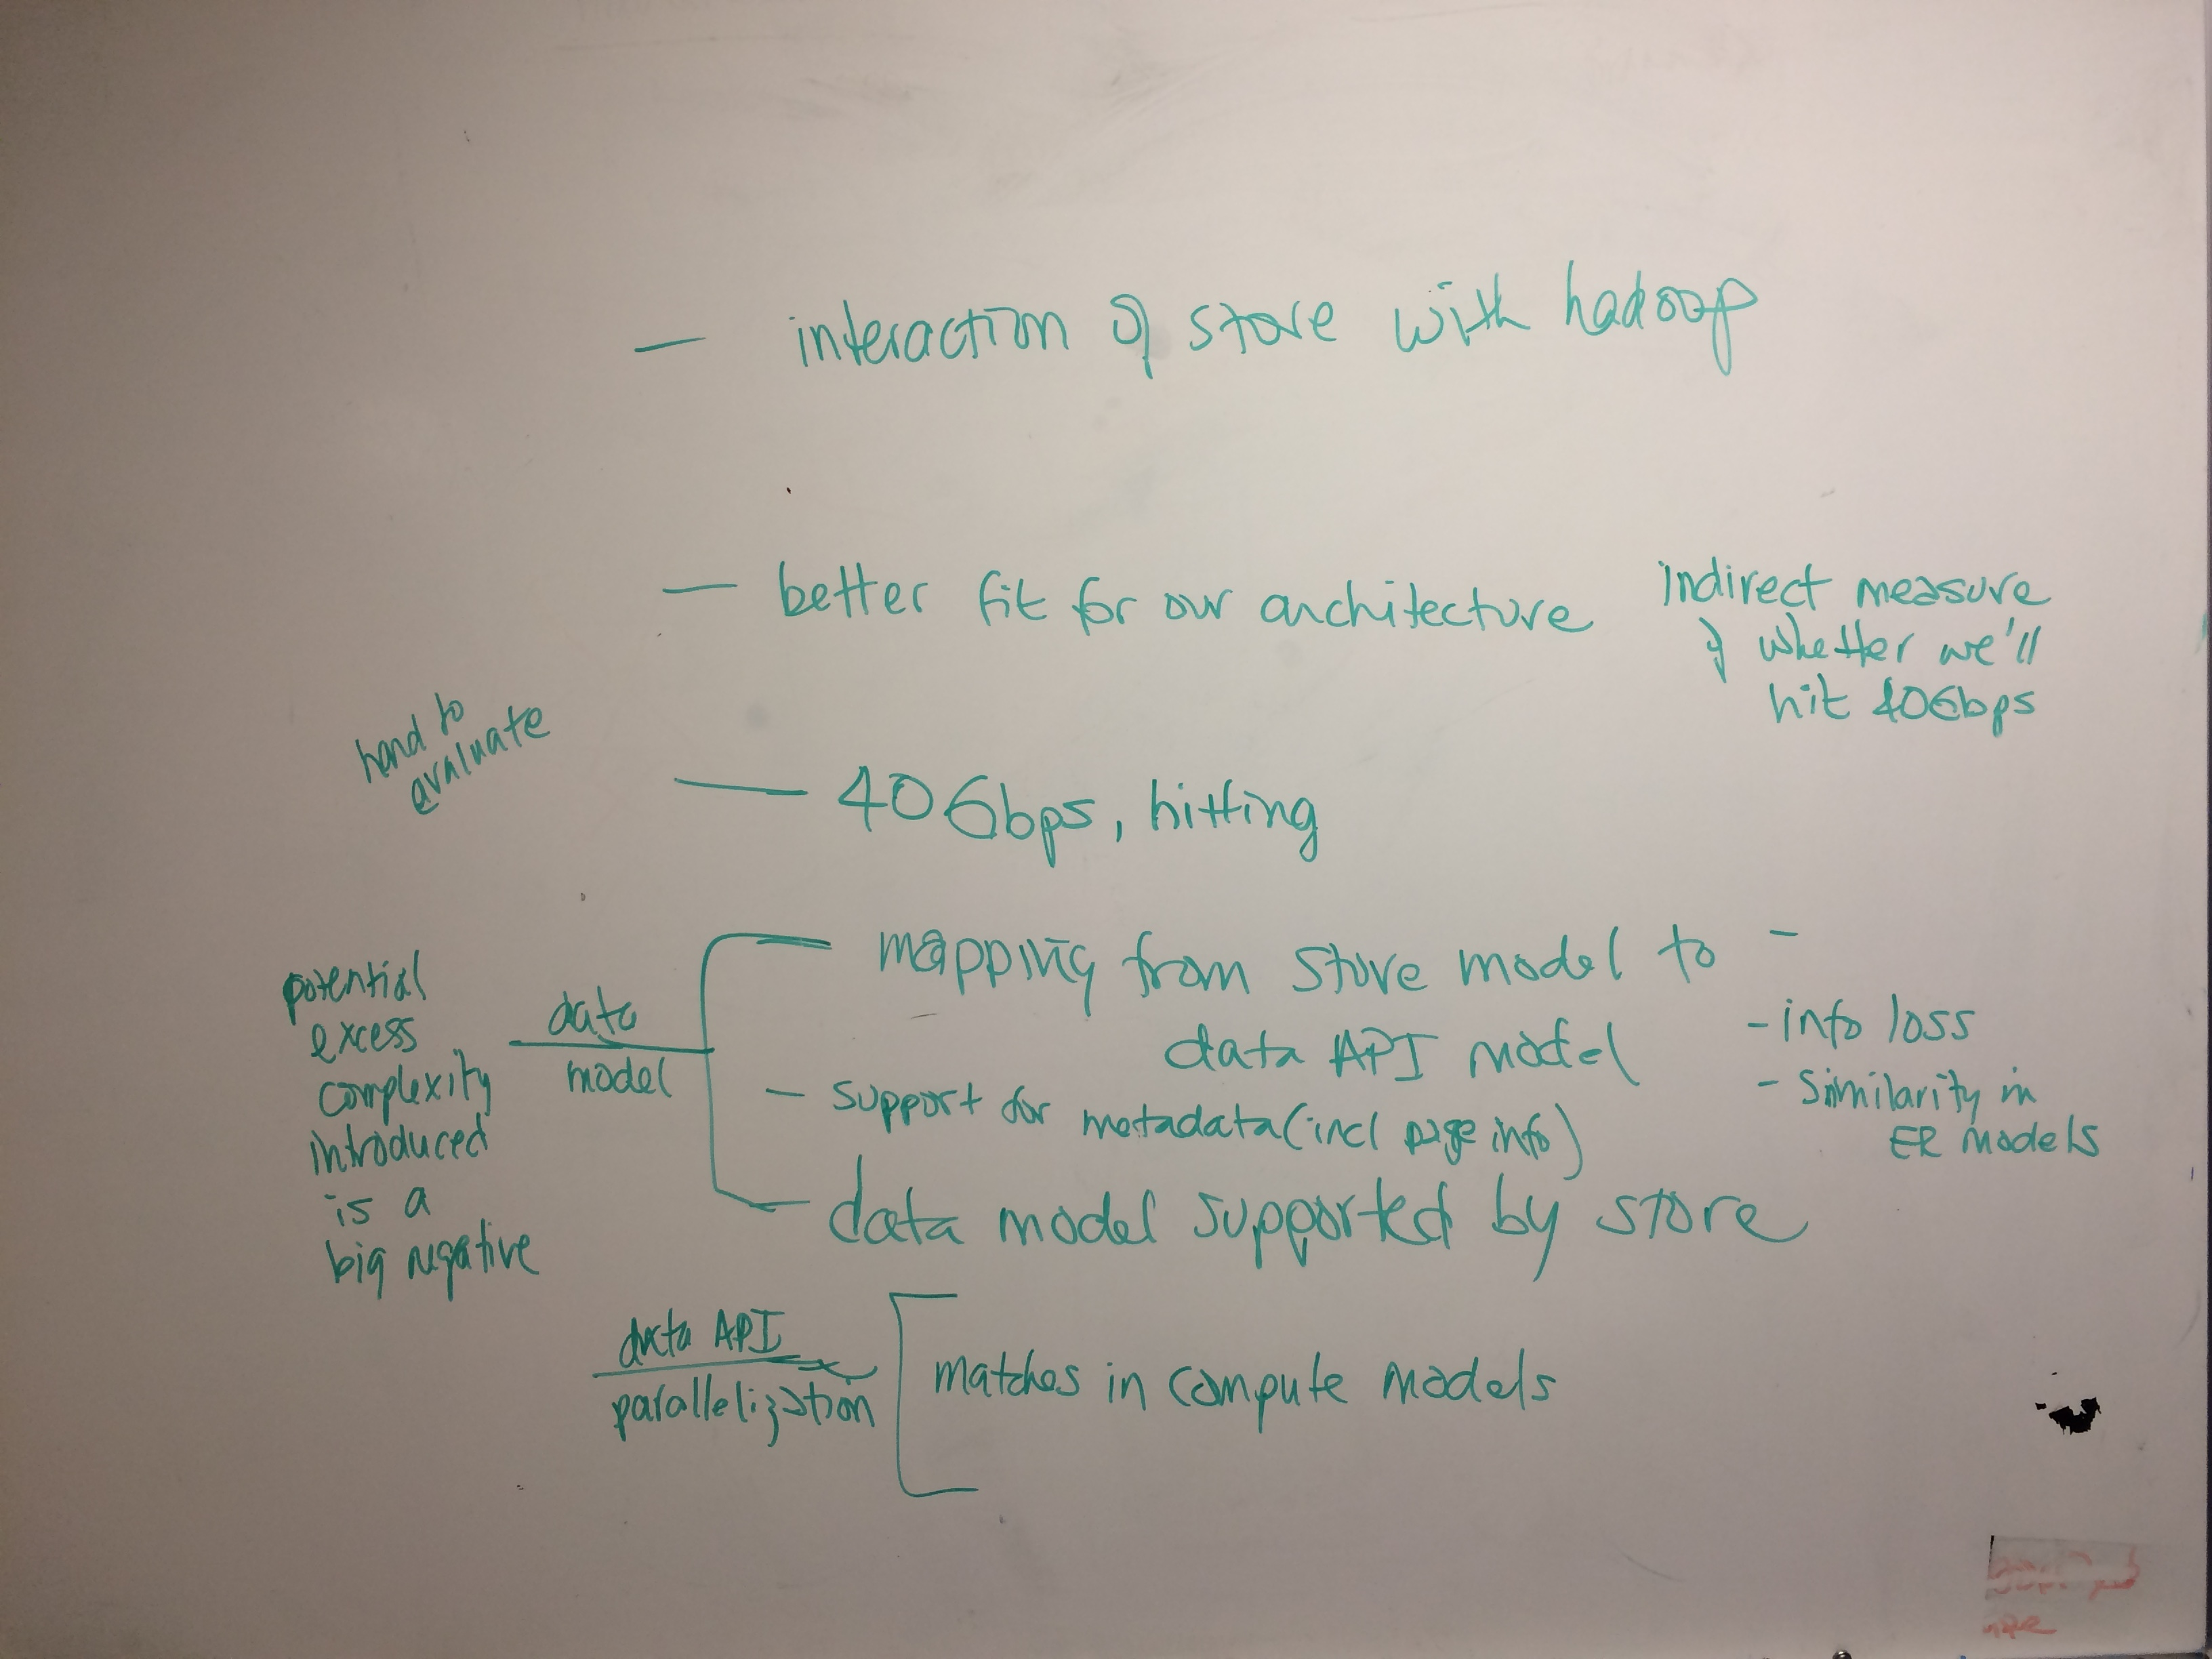
\includegraphics[width=0.95\textwidth]{IMG_0475}
    \caption{Notes from the July 13th discussion (Milinda and Beth)}
    \label{fig:notes}
\end{figure}


\bibliographystyle{abbrv}
\bibliography{references}

\end{document}